% !TeX spellcheck = de_DE
%\documentclass[11pt,a4paper]{article}
\documentclass[11pt
  , a4paper
  , article
  , oneside
%  , twoside
%  , draft
]{memoir}
\setcounter{secnumdepth}{2}
\usepackage{control}
\usepackage[numbers]{natbib}

\newcommand{\newappendix}{%
	\refstepcounter{chapter}\chapter*{Appendix \thechapter}%
	\addcontentsline{toc}{chapter}{Appendix \thechapter}%
}

\newcommand\tab[1][1cm]{\hspace*{#1}}

\begin{document}

\newcommand{\technumber}{
  RAON Control-Document Series\\
  Revision : v1.0,   Release : 2016-12-02 fixed date}
\title{\textbf{EPICS V4 PVAccess Gateway 프로토타입 개발 결과보고서}}

\author{이상일\thanks{silee7103@ibs.re.kr} \\

  Rare Isotope Science Project\\
  Institute for Basic Science, Daejeon, South Korea
}
\date{\today}

\renewcommand{\maketitlehooka}{\begin{flushright}\textsf{\technumber}\end{flushright}}
%\renewcommand{\maketitlehookb}{\centering\textsf{\subtitle}}
%\renewcommand{\maketitlehookc}{C}
%\renewcommand{\maketitlehookd}{D}

\maketitle

\begin{abstract}
본 문서는 EPICS Version 4 통신 프로토콜 "pvAccess"를 정의하고, 그에 따른 "pvAccess Gateway"의 프로토타입 개발 구현에 대한 결과를 설명하는 보고서이다. 또한 본 문서의 pvAccess Gateway 프로토타입 개발은 RAON 중이온가속기에서의 초기 개발 비용을 시작으로 다른 해외연구기관이 그를 이어 받아 향 후 안정화 운영시기까지 계속적인 개발 및 버전 업데이트가 이루어 질 예정이다. 
\end{abstract}

EPICS\citep{epics}는 대형실험 과학 장치의 제어시스템을 구축하기 위한 모든 컴퓨터의 플랫폼으로 정의된다. 또한, 더욱 넓은 의미로, EPICS는 EPICS community에서 공동으로 개발되고 전 세계에서 실시간 분산 소프트웨어 제어 시스템을 작성하는데 사용되는 일련의 오픈 소스 소프트웨어 도구, 라이브러리 및 응용 프로그램이기도 하다. 그 중 EPICS version4\citep{epics_v4}의 pvAccess\citep{epics_v4_pvaccess}는 계측센서 신호에 대한 모니터링 및 과학적 데이터 서비스를 상호 연결하는 고성능 네트워크 통신 프로토콜을 말한다. 이는 제어시스템의 양끝단의 최적화된 내부통신을 위해서 pvData라는 EPICS version 4 공유메모리 기반의 통신 오브젝트 객체로써, 구조화된 사용자 정의 데이터 타입을 지원하며, EPICS version 3 "channel access" 프로토콜을 계승한다. EPICS V4 pvAccess 프로토콜 및 기본 구현은 EPICS 워킹그룹에 의해 작성된다. pvAccess gateway의 클라이언트를 "외부"로 지칭하며, 게이트웨이 외부 클라이언트를  연결하는 서버 (예:IOC)를 "내부"로 지칭한다. 이는 게이트웨는의 양면 사이를 명확히 구별하기 위함이다. EPICS에 대한 자세한 내용은 "Experimental Physics and Industrial Control System"\citep{epics}의 홈 페이지를 참조한다. 

\clearpage

\chapter{EPICS v3 Channel Access Gateway}
pvAccess gateway를 이해하기 위하여, EPICS V3의 channel access 기반의 gateway에 대한 기본특성을 설명한다.

\section{특성}
EPICS V3 channel access 통신프로토콜은 TCP/IP 기반의 서버/클라이언트 통신 구조를 갖는다. 이러한 구조에서 사용자측에서 EPICS IOC 서버에 데이터 요청이 있을 경우에 대하여 Flat한 네트워크상에서 연결이 이루어진다면 Figure \ref{fig:flat_network}과 같은 구성이된다. 이러한 구성은 EPICS IOC 서버단에서 통신 연결에 대한 리소스를 많이 부담해야 하고, 동일한 데이터 패킷이 네트워크 상에 중복 분포되어 네트워크 부하를 유발하는 원인이 된다.
 
\begin{figure}[!htb]
	\centering
	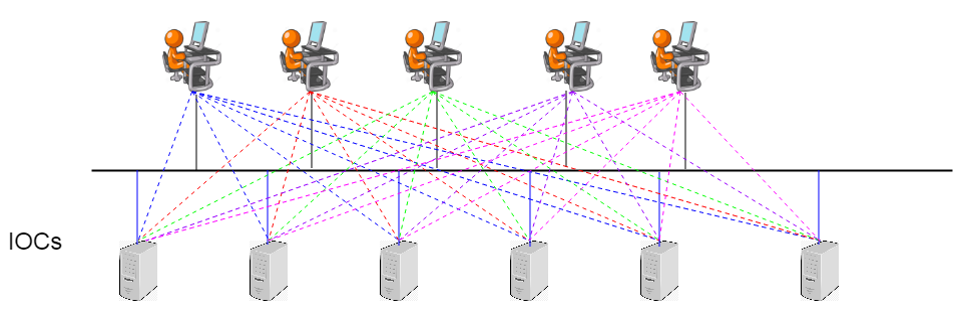
\includegraphics[width=1\textwidth]{./images/flat_network.png}
	\caption{
		Flat Network 상에서의 문제점
	}
	\label{fig:flat_network}   
\end{figure}

이런 문제 발생을 사전에 막기위하여 proxy 서버 역할 및 네트워크 연결을 효율적으로 관리하는 software 가 필요하다. 

\section{Channel Access Gateway 구성 및 주요기능}
EPICS V3 channel access gateway는 Figure \ref{fig:gateway}와 같이 네트워크를 계층적, 물리적으로 나누어 구성 할 수 있다. 이와 같은 proxy 서버의 역할을 위한 gateway는 channel access 통신 프로토콜의 server 역할 및 client 역할을 모두 수행 할 수 있어야 한다. 즉, OPI를 바라보는 입장에서는 channel access server 역할을 IOC를 바라보는 입장에서 channel access client 역할을 수행한다. 주요 channel access 기능을 살펴보면 아래와 같다.

\begin{itemize}
	\item TCP/IP Communication management
	\item Caching of Process Variable for data deduplication.
	\item Aliasing for Process Variable name
	\item Access Security for PV name
	\item Report for connection status
\end{itemize}
 
\begin{figure}[!htb]
	\centering
	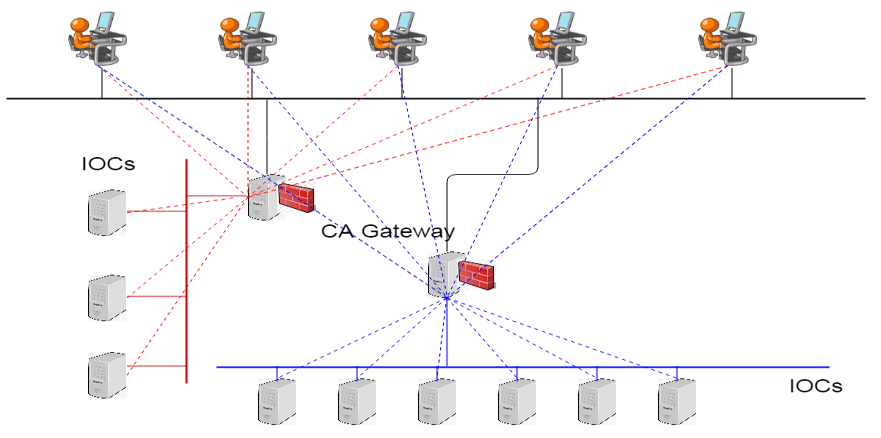
\includegraphics[width=1\textwidth]{./images/gateway.png}
	\caption{
		Gateway 구성
	}
	\label{fig:gateway}   
\end{figure}

상위 Figure \ref{fig:gateway}와 같이 gateway는 계층적, 물리적 분리된 네트워크 상에 최적화된 네트워크 연결 구성 및 접근 보안성을 통하여 효율적인 제어 네트워크 구성을 가능하게 한다.


\chapter{EPICS v4 PVAccess Gateway Prototype}
\section{EPICS Version 4 pvAccess}
EPICS Version 4의 pvAccess 통신프로토콜은 Version 3의 Channel Access 통신프로토콜의 제한 사항을 확장 시킨 프로토콜이다.EPICS Version 4는 기존 EPICS Version 3에 추가적으로 복잡한 scientfic complex 데이터 구조를 사용자 정의가 가능하도록 구현되는 Service 관점의 아키텍쳐로 확장된다. EPICS version 4는 현재 EPICS 버전 중 성능에 있어서 가장 우수하며, 분산 데이터 수집, 서비스 지향 아키텍처 및 복잡한 데이터 구조를 지원합니다. EPICS v4 워킹 그룹은 EPICS v4 기반 프로토콜 및 소프트웨어의 표준에 대한 참조 구현 및 정의를 제공하기 위한 노력을 기울인다. 
\hfil\break\hfil\break
EPICS v4는 EPICS base에 아래와 같은 주요기능이 추가 되었다.
\begin{itemize}
	\item 사용자 정의 complex data I/O 확장(Image data 및 HDF5 file format)
	\item High-performance streaming
	\item New front-end processing database for managing complex data
	\item Synchronous RPC(Remote Procedure Call) for service-oriented architecture
	\item Asnynchronous device/driver support
	\item Data processing pipeline
\end{itemize}

EPICS version4는 수많은 표준 C++/Java APIs 라이브러리로 구성되며, 다른 EPICS 구성요소 및 툴들과 연동 될 수 있다. 이러한 목적은 public-review 과정을 통하여 공개된 표준 APIs이 플랫폼에 독립적으로 구현 될 수 있게 하기 위함이며, 이에 충실히 따른 개발로 진행되었다.

\section{동기 및 특성}
EPICS v3의 CA(channel access) gateway 구성요소와 유사하게 EPICS v4 PV(PVAccess) gateway 구성요소는 CA(v3)와 PV(v4)로 명명된 클라이언트 및 서버를 포함한 어플리케이션을 말한다. 그것의 주된 기능은 IP 네트워크 경계를 가로지르는 proxy connection 이다. 이는 gateway의 클라이언트 측에서 서버(IOC) 를 보호하기 위하여 채널 이름을 고유하게 해석하고, 데이터 update를 클라이언트로 보내는 작업을 gateway 측으로 옮기는 역할을 한다. 이를 위하여 PV gateway는 더많은 네트워크 연결 및 컴퓨터 자원 할당이 가능한 장치가 사용되어야 한다. 

\section{기능 요구사항}
\subsection{요구사항 ID}
pvAccess gateway에 대한 요구사항\cite{epics_v4_requirement} ID는 아래와 같은 포맷으로 정의된다.
 \newline
\hfil\break

PVGW-REQ-\{req-category\}-\{req-number\} \newline

\begin{center}
	\begin{longtable}[t]{>{\raggedleft\arraybackslash} p{3cm} |p{2cm}}
		\caption{Requirement Category}
		\label{table:req_cat}\\
		\toprule
		\texttt{Category} & \textbf{ID} \\
		\midrule
		\endfirsthead
		\toprule
		\texttt{Category} & \textbf{ID} \\
		\midrule
		\endhead
		\midrule \multicolumn{2}{r}{\tablename\ \thetable\ -- \textit{Continued on next page}} \\
		\bottomrule
		\endfoot
		\bottomrule
		\endlastfoot
		\texttt{Functional}  & F \\
		\texttt{External}  & I \\
		\texttt{Other}    & O \\
	\end{longtable}
\end{center}

\subsection{EPICS Network Protocol 요구사항}
\subsubsection{PVGW-REQ-F-001 pvAccess Client}
The Gateway should be able to connect to internal servers using the pvAccess network protocol of EPICS V4.

\subsubsection{PVGW-REQ-F-002 pvAccess Server}
The Gateway should provide channels on the external network by means of the pvAccess network protocol of EPICS V4.

\subsubsection{PVGW-REQ-F-003 Configurable pvAccess Server}
It should be possible to configure if the pvAccess server (PVGW-REQ-F-002) is started. This configuration should be defined at start-up, and is not required to be changeable at runtime.

\subsubsection{PVGW-REQ-F-004 Redundant pvAccess Server Operation}
It should be possible to run multiple Gateways with identical configuration in parallel, to allow failover and load balancing. This mode should not require special configuration on the external clients.

\subsubsection{PVGW-REQ-F-011 Channel Access Client}
The Gateway should be able to connect to internal servers using the Channel Access network protocol of EPICS V3.

\subsubsection{PVGW-REQ-F-012 Channel Access Server}
The Gateway should provide channels on the external network by means of the Channel Access network protocol of EPICS V3.

\subsubsection{PVGW-REQ-F-013 Configurable Channel Access Server}
It should be possible to configure if the Channel Access server (PVGW-REQ-F-012) is started. This configuration should be defined at start-up, and is not required to be changeable at runtime.

\subsubsection{PVGW-REQ-F-021 Configurable Server Side Network Binding}
On machines with multiple network interfaces, the Gateway should allow configuration of the network interfaces that its server(s) bind to. This configuration should be defined at start-up, and is not required to be changeable at runtime.


\subsection{Data Flow Engine 요구사항}
\subsubsection{PVGW-REQ-F-101 Full pvData Support}
The Gateway should support transport of all pvData structures without restrictions. No legal pvData type should require recompilation or restart of the Gateway.

\subsubsection{PVGW-REQ-F-102 Full Normative Type Support}
The Gateway should support transport of all Normative Type (NT) structures without restrictions. it must not depend on specific properties of any NT.

\subsubsection{PVGW-REQ-F-111 Low Latency for Large Structures/Arrays}
The Gateway should add minimal latency when forwarding large structures or arrays. Sending data to the external clients should start immediately, and not require data structures to be received completely.

\subsubsection{PVGW-REQ-F-112 Quality-of-Service Mechanisms}
The Gateway should implement mechanisms to avoid negative effects of connections with large structures and arrays on connections to other PVs on the same internal server.

\subsubsection{PVGW-REQ-F-121 Combine Sub-Structure Subscriptions}
The Gateway should be able to combine external clients' subscriptions to different sub-structures of the same channel into one subscription to the internal server.

\subsubsection{PVGW-REQ-F-122 Combine Request Configurations for Identical Subscriptions}
The Gateway should be able to combine external clients' request configurations (pvRequest) for subscriptions to identical sub-structures of the same channel into one subscription to the internal server.

\subsubsection{PVGW-REQ-F-131 Data Cache}
The Gateway should be able to cache data, so that data for replies to get operations and initial updates on new subscriptions from external clients may be taken from the cache.

\subsubsection{PVGW-REQ-F-132 Configurable Data Cache}
Application of the "Data Cache" feature (PVGW-REQ-F-131) to get operations should be configurable, both globally and specifically on a channel name/regex base.

\subsubsection{PVGW-REQ-F-141 Transparent Data Behavior}
The Gateway should act completely transparent. When comparing a direct connection to a PV with a connection through the Gateway, order and contents of received data should be the same.
This does not apply to get operations, when data caching (PVGW-REQ-131) is enabled. In that case, the values returned from the cache may be different from the values in the internal server

\subsubsection{PVGW-REQ-F-142 Transparent Out-of-Band Behavior}
The Gateway should act transparent with respect to out-of-band behavior. When comparing a direct connection to a PV with a connection through the Gateway, out-of-band situations (e.g., connection loss, reconnection, non-existent PV) should produce the same exceptions in the same order.

\subsubsection{PVGW-REQ-F-143 Transparent Timeout Behavior}
The Gateway should act transparent with respect to timeouts. When comparing a direct connection to a PV with a connection through the Gateway, timeouts defined by the external client should be honored in the same way.

\subsubsection{PVGW-REQ-F-151 Name Server}
If the Gateway receives a name resolution request from an external client for a channel that it already serves, it should send an immediate positive reply to the request without querying the internal servers. If the Gateway receives a name resolution request from an external client for a channel that it should serve, but lost connection to, it should send an immediate negative reply to the request without querying the internal servers. If the Gateway receives a name resolution request from an external client for a channel that it was not able find recently (within a configurable interval), it should send an immediate negative reply to the request without querying the internal servers.

\subsubsection{PVGW-REQ-F-161 Connection Cache}
The Gateway should cache connections, i.e. keep the channel connection open with subscription disabled, for a configurable time after the last external client disconnected.


\subsection{Authentication/Authorization 요구사항}

\subsubsection{PVGW-REQ-F-201 Local AuthN/AuthZ}
The Gateway should support a local layer of authentication and authorization, where authN/authZ for requests is decided possibly using an independent authN/authZ server, but without querying the internal server.
항
\subsubsection{PVGW-REQ-F-202 Run-Time Configurable Local AuthN/AuthZ}
The "Local AuthN/AuthZ" feature (PVGW-REQ-F-201) should be configurable at run-time. Activating a new configuration should not require a restart of the Gateway. Connections whose authZ does not change by the new configuration should not be affected.

\subsubsection{PVGW-REQ-F-203 Proxy AuthN/AuthZ}
The Gateway should support proxy authentication and authorization, where authorization for requests is decided by querying the internal server, using the credentials supplied by the external client.

\subsubsection{PVGW-REQ-F-211 Transparent AuthZ Forwarding}
The Gateway should transparently forward authorization changes on the internal connections to its external clients.

\subsection{External Interface 요구사항}
\subsubsection{PVGW-REQ-I-001 Statistics Data}
The Gateway should provide statistical and performance data as pvData NT structures.

\subsubsection{PVGW-REQ-I-002 Network Binding for Statistics Data}
On machines with multiple network interfaces, the Gateway should allow configuration of the network interfaces that the statistics data (PVGW-REQ-I-001) server(s) bind to, independent from the equivalent setting of the data server(s) (PVGW-REQ-F-021). This configuration should be defined at start-up, and is not required to be changeable at runtime.항
\subsubsection{PVGW-REQ-I-011 Debugging Shell}
The Gateway should provide a shell for debugging purposes, allowing to inspect its internal structures and lists, trace requests, set up debug log output filtered by channel or external client or internal server, etc.

\subsection{Other 요구사항}
\subsubsection{PVGW-REQ-O-001 Build Environment}
The Gateway component should compile in a standard EPICS V4 build environment, using the standard EPICS V4 tools and compilers.

\subsubsection{PVGW-REQ-O-002 Supported Platforms}
The Gateway should be supported on all host type architectures/platforms officially supported by EPICS V4.

\subsubsection{PVGW-REQ-O-003 SMP Support}
The Gateway should be able to make use of SMP architectures, distributing load onto the available CPUs.

\section{PVAccess Gateway 프로토타입 설계 및 구현}
\subsection{PVAccess Server/Client Connection}
pvAccess gateway는 앞서 설명한대로 통신에서의 server와 client 역할을 동시에 수행한다. Figure \ref{fig:connections}에서 보듯이 다수의 OPI(OPerator Interface)의 clients들은 gateway의 GWS server에 연결되며, gateway의 GWC client는 EPICS IOC SRV에 연결되는 구조로 일종의 proxy server 역할을 수행한다. 이후 gateway의 GWS 및 GWC의 내부 로직에 의한 processing이 이루어진다. 

\begin{figure}[!htb]
	\centering
	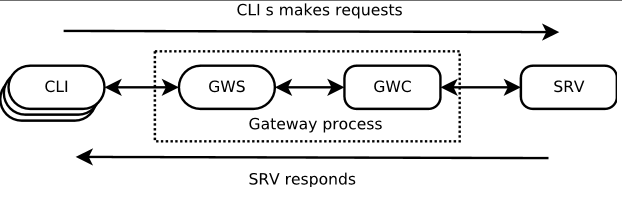
\includegraphics[width=0.5\textwidth, height=0.2\textheight]{./images/connections.png}
	\caption{
		PVAccess Gateway 구조
	}
	\label{fig:connections}   
\end{figure}

\subsection{PVAccess Gateway Sequence}
Figure \ref{fig:search}에서와 같이 CLI\#1에서 PV(Process Variable)를 요청을 의뢰하면 gateway의 GWS는 해당 unicast 메시지를 받아 cache list를 검색한다. 해당 list에서 cache hit을 실패하면 GWC는 해당 unicast 메시지를 설정된 SRV에 포워딩하거나 broadcast 메시지를 전송한다. 각 끝단의 EPICS IOC SRV들 중에서 전송된 메시지에 해당하는 PV를 가지고 있다면 해당 PV에 대하여 응답메시지를 gateway의 GWC에 전달한다. 이때 gateway의 GWC는 해당 IOC SRV에 RPC(Remote Procedure Call) 채널 연결을 요청하고 이에 대해 connection을 맺은 후 gateway의 cache list에 추가하며, CLI\#1에 RPC 통신연결을 수락한다. 이후 cycle 부터는 cache hit에 의한 PV 데이터를 획득한다. 동시에 CLI\#2에서 CLI\#1에서 요청하였던 PV에 대하여 요청 할 경우 gateway의 GWS는 cache hit에 의해 바로 CLI\#2에 해당 PV 데이터를 응답하여 전송한다. 이후 설정된 PV 데이터의 경우 IOC SRV는 변경된 데이터에 대하여 event메시지를 발생하며, gateway의 GWC는 해당 event를 queue에 넣는다. gateway GWS는 해당 queue list에서 해당 PV 데이터를 pop하여 연결 설정된 CLI\#1 및 CLI\#2에 PV 데이터를 전송한다. 

\begin{figure}[!htb]
	\centering
	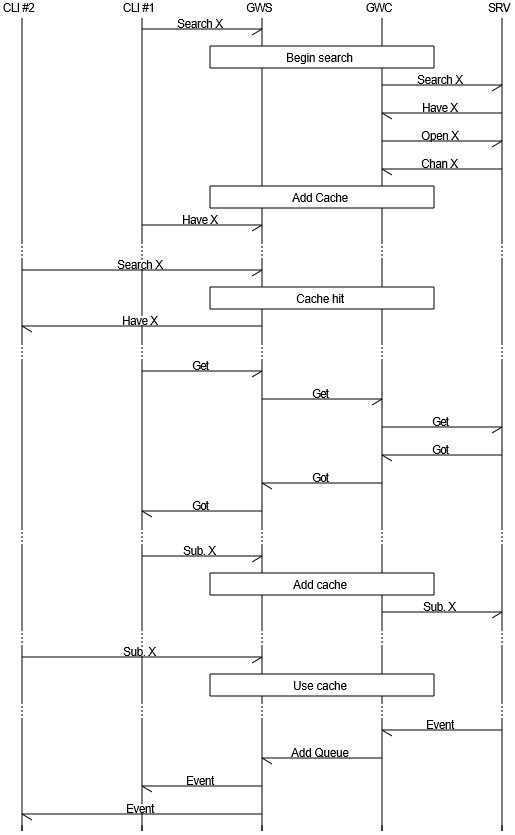
\includegraphics[width=0.8\textwidth, height=0.7\textheight]{./images/search.png}
	\caption{
		Search Logic Time Line 차트
	}
	\label{fig:search}   
\end{figure}

\clearpage

Figure \ref{fig:cached}는 client에서 gateway의 GWS에 연결시 cache list를 관리하는 순서를 보여준다. client에서 PV 데이터 요청시 해당 PV 이름을 key 값으로 하는 cache hash list에서 key값에 대해 cache miss가 발생하거나 chach list에는 존재하나 실제 IOC SRV와 RPC channel connection이 없다면 RPC channel connection이 이루어진다. 이후 gateway의 GWC는 IOC SRV로 부터 데이터를 받아 cache update를 수행한다. 이후 모든 client는 해당 PV 데이터에 대하여 cached 된 데이터를 사용하게 된다.

\begin{figure}[!htb]
	\centering
	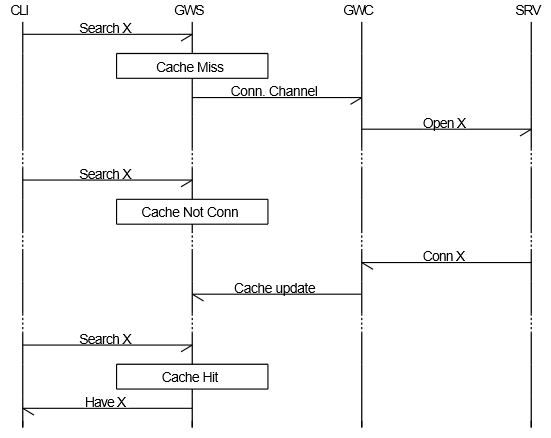
\includegraphics[width=0.6\textwidth, height=0.4\textheight]{./images/cached.png}
	\caption{
		PVAccess Gateway Cache Logic
	}
	\label{fig:cached}   
\end{figure}

Figure \ref{fig:workflow}는 template 기반의 modern c++ gateway를 구현한 개체의 instance 생성 및 process 흐름도를 보여준다. 주요 context 흐름을 살펴보면 gateway 실행시 ServerContextImpl 개체의 instance를 통하여 GWServerChannelProvider instance 개체가 생성되며 이는 server와 client 사이에서 ChannelCacheEntry instance를 통하여 gateway에 대한 통신 및 PV 데이터에 대한 monitoring event에 대한 channel cache list를 관리한다. GWChannel 개체의 instance는 CLI에서 요청하는 PV에 대하여 RPC channel connection 관리한다.

\begin{figure}[!htb]
	\centering
	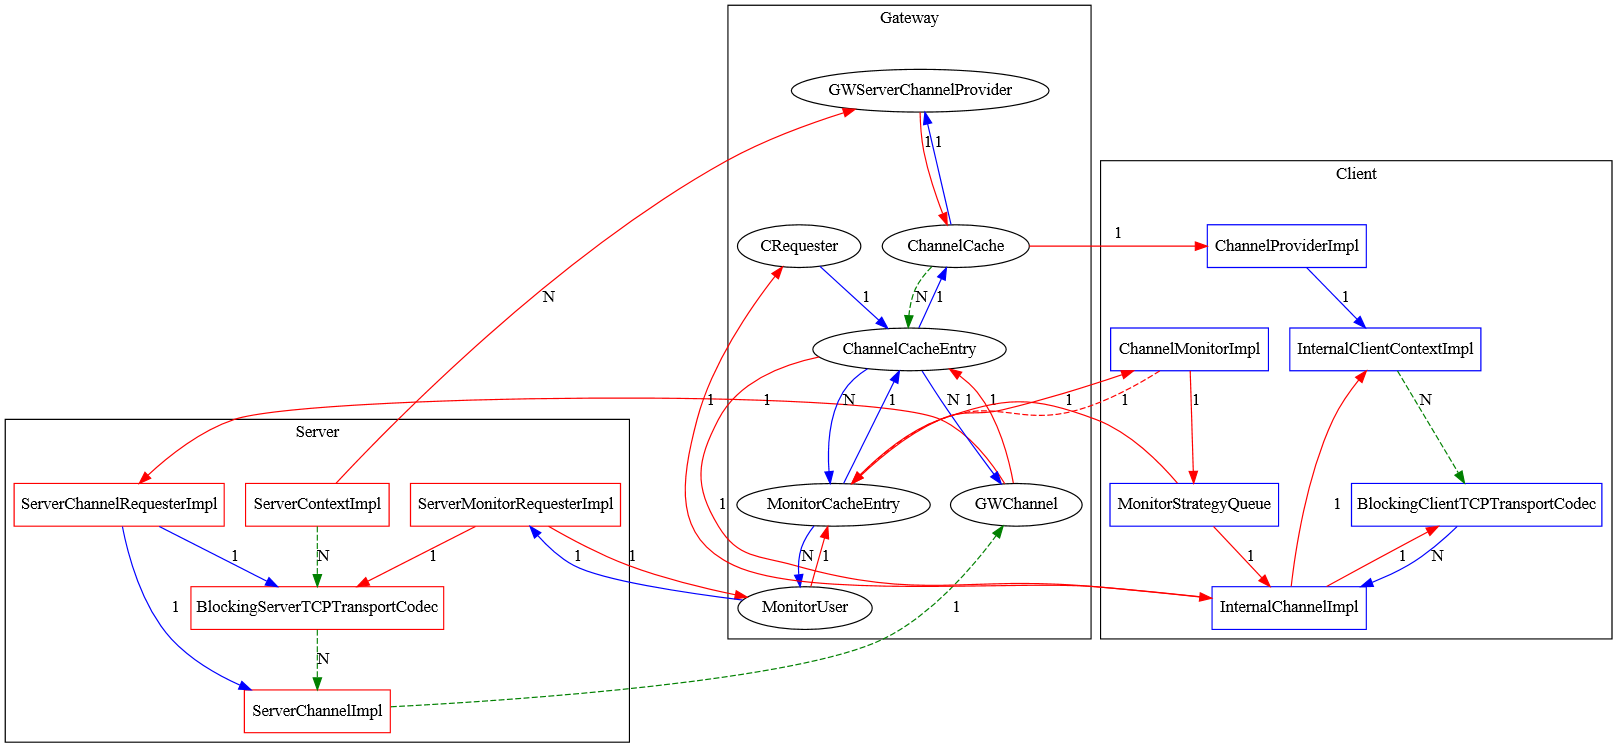
\includegraphics[width=1\textwidth, height=0.7\textheight]{./images/work_flow.png}
	\caption{
		PVAccess Gateway Process Flow
	}		
	\label{fig:workflow}   
\end{figure}

\clearpage

\section{시험 결과}
\subsection{PVAccess Gateway 주요 환경변수}
pvAccess Gateway prototype 구성 시험환경을 위하여는 EPICS v4 pvAccess에 관련한 주요 환경변수를 아래와 같이 설정한다.

\begin{lstlisting}[style=termstyle]
# PVA variables

# Server side
#
# EPICS_PVAS_INTF_ADDR_LIST - Bind to this interface for both UDP and TCP
# EPICS_PVAS_SERVER_PORT - default TCP port
# EPICS_PVAS_BROADCAST_PORT - Listen for searches on this port
# EPICS_PVA_SERVER_PORT - Unused if EPICS_PVAS_SERVER_PORT set
#
# Client side
#
# EPICS_PVA_BROADCAST_PORT - Default search port for *ADDR_LIST
# EPICS_PVA_ADDR_LIST - Space seperated list of search endpoints (bcast or unicast)
# EPICS_PVA_AUTO_ADDR_LIST - YES/NO whether to populate ADDR_LIST with all local interface bcast addrs


\end{lstlisting}

\subsubsection {EPICS\_PVAS\_INTF\_ADDR\_LIST = 10.1.5.50}
pvAccess gateway GWS 서버에서 UDP 및 TCP 소켓통신과 Binding하기 위한 IP 주소를 설정하기 위하 환경변수 이다.

\subsubsection {EPICS\_PVA\_ADDR\_LIST = 10.1.4.61}
pvAccess gateway GWC 클라이언트에서 EPICS IOC와 pvAccess 통신 프로토콜 설정을 위한 endpoints IP 어드레스 리스트를 설정하는 환경변수 이다. 환경변수에 정의된 IP 리스트에 unicast 메시지 또는 broadcast 메시지를 전송한다.

\subsubsection {EPICS\_PVA\_AUTO\_ADDR\_LIST=No}
pvAccess gateway GWC 클라이언트에서 EPICS IOC와 pvAccess 통신 프로토콜 설정을 위하여 EPICS\_PVA\_ADDR\_LIST에 정의된 IP에 대하여 unicast 메시지만을 보낼지 또는 추가적으로 자신의 네트워크 subnet mask에 설정된 주소에 broadcast 메시지를 보낼지를 선택하는 환경변수 이다.


\subsubsection {EPICS\_PVAS\_SERVER\_PORT}
pvAccess gateway 서버에서 TCP 통신포트를 설정하기 위한 환경변수 이다. 디폴트(5064) 포트를 사용한다.

\subsubsection {EPICS\_PVAS\_BROADCAST\_PORT}
pvAccess gateway 서버에서 각 클라이언트에서 PV search에 대한 UDP 메시지를 받기 위한 UDP 통신포트 설정 환경변수 이다. 디폴트 포트를 사용한다.

\subsubsection {EPICS\_PVA\_ADDR\_LIST = 10.1.5.50}
OPI(OPerator interface)의 클라이언트에서 pvAccess gateway GWS 서버 주소를 설정하기 위한 환경변수 이다.

\subsubsection {EPICS\_PVA\_AUTO\_ADDR\_LIST=No}
OPI(OPerator interface)의 클라이언트에서 자신의 네트워크 subnet mask에 설정된 주소에 broadcast 메시지를 보낼지를 선택하는 환경변수 이다.

\subsection{PVAccess Gateway Prototype 환경구성 및 시험}
Figure \ref{fig:gw_env}는 pvAccess gateway prototype 시험을 위하여 설정된 환경구성이다. pvAccess gateway(10.1.5.50)는 분리된 네트워크(10.1.4.x, 10.1.5.x)에서 proxy 서버의 역할을 수행한다. 

\begin{figure}[!htb]
	\centering
	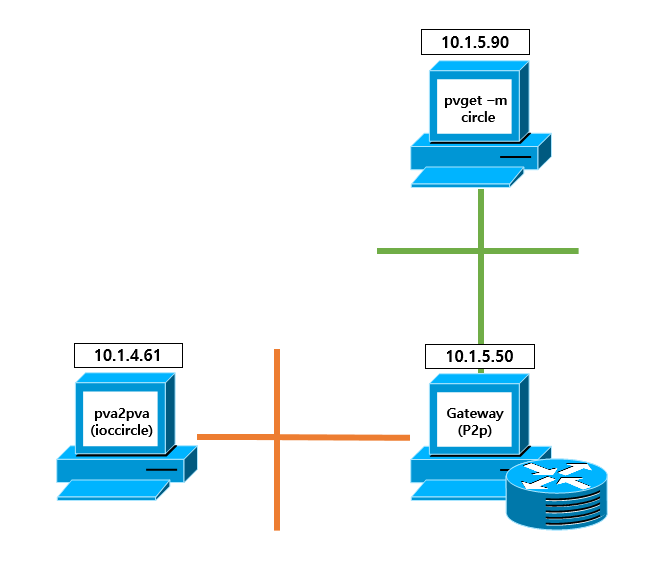
\includegraphics[width=0.6\textwidth, height=0.4\textheight]{./images/gw_env.png}
	\caption{
		PVAccess Gateway Prototype 시험환경 구성
	}		
	\label{fig:gw_env}   
\end{figure}


\clearpage
\subsubsection{EPICS PVAccess IOC SRV 실행}
Figure \ref{fig:ioc}에서 처럼 10.1.4.61번의 IOC SRV에서 pvAccess에 대한 EPICS IOC를 실행한다. 

\begin{figure}[!htb]
	\centering
	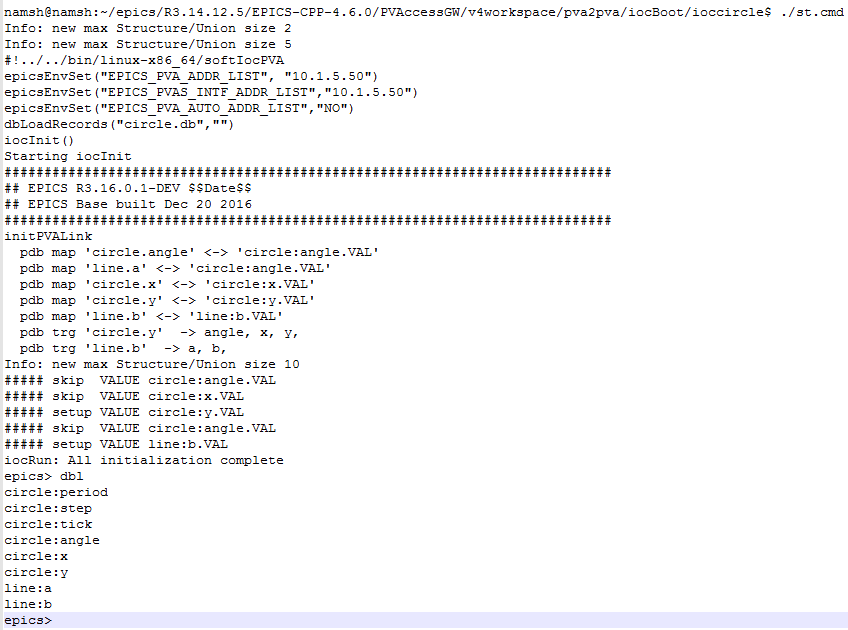
\includegraphics[width=0.8\textwidth, height=0.5\textheight]{./images/ioc.png}
	\caption{
		EPICS IOC SRV 실행(10.1.4.61)
	}		
	\label{fig:ioc}   
\end{figure}

\clearpage


\subsubsection{PVAccess Gateway 실행}
Figure \ref{fig:gw_start}에서 처럼 10.1.5.50번에서 pvAccess에 대한 gateway를 실행한다. 

\begin{figure}[!htb]
	\centering
	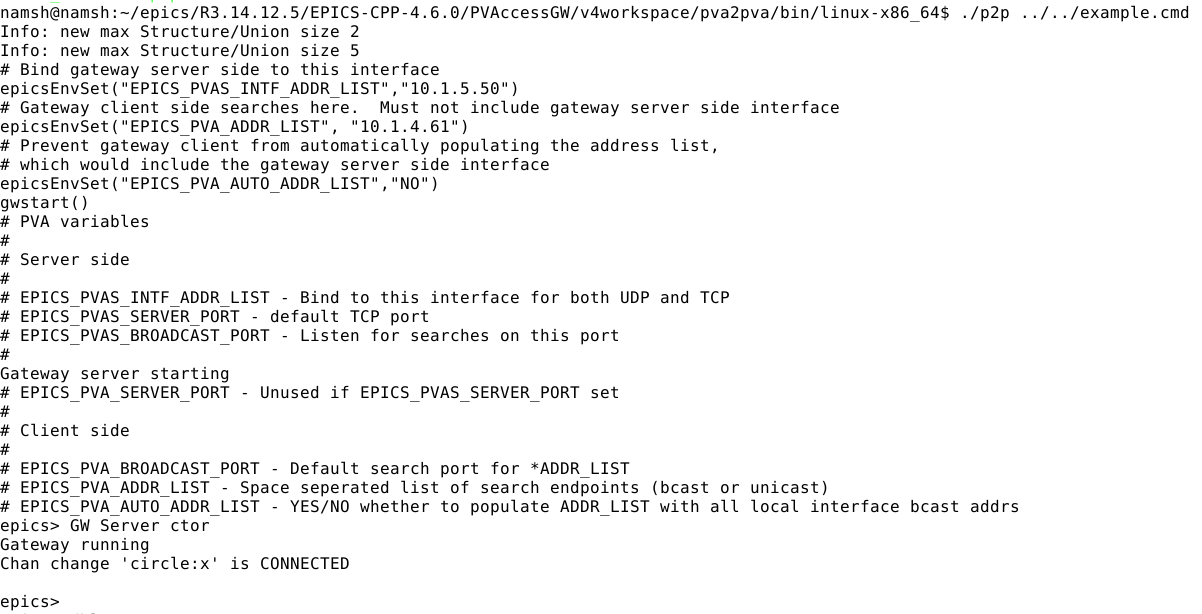
\includegraphics[width=0.8\textwidth, height=0.5\textheight]{./images/GW_start.png}
	\caption{
		pvAccess gateway 실행(10.1.5.50)
	}		
	\label{fig:gw_start}   
\end{figure}
\clearpage


\subsubsection{PVAccess Data 검증}
Figure \ref{fig:pvget}에서 처럼 10.1.5.60번에서 pvAccess 프로토콜을 사용한 데이터가 액세스 되는지 아래 명령어를 통해 확인한다.

Figure \ref{fig:pvget}의 왼쪽 화면은 예로 사용된 circle 이라는 사용자가 정의 가능한 복잡한 데이터 타입(normativeTypes)에 따른 pvAccess data를 획득하는 예이며, 오른쪽 화면은 circle의 여러 데이터 중 스칼라 형의 데이터를 개별적으로 획득하는 화면을 보여준다.


\begin{lstlisting}[style=termstyle]
~pvAccess/bin/linux-x86_64$>./pvget -m circle
~pvAccess/bin/linux-x86_64$>./pvget -m circle:x circle:y circle:angle
\end{lstlisting} 

\begin{figure}[!htb]
	\centering
	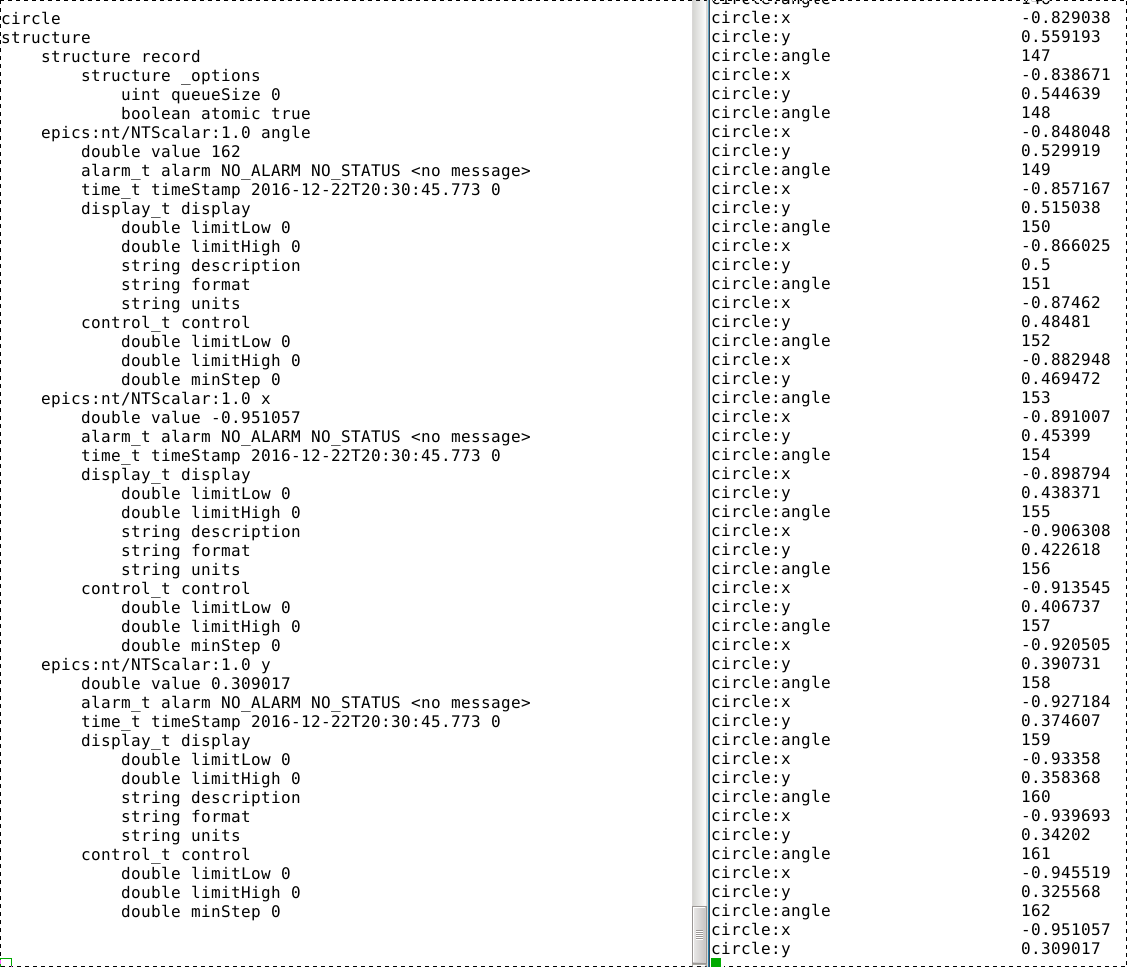
\includegraphics[width=0.8\textwidth, height=0.5\textheight]{./images/pvget_result.png}
	\caption{
		pvget pvname(10.1.5.60)
	}		
	\label{fig:pvget}   
\end{figure}

\clearpage
\subsubsection{Gateway Message}
Figure \ref{fig:gw_msg}에서 처럼 gateway에서 출력되는 메시지는 앞서 설명한대로 gateway 가 cache hash list를 관리하며 pvAccess 데이터가 중복 요청이 될 경우 cache hit이 발생하며 처음 요청되는 pvAccess의 경우 cache miss를 통해 새로운 channel이 이루어진다.

\begin{figure}[!htb]
	\centering
	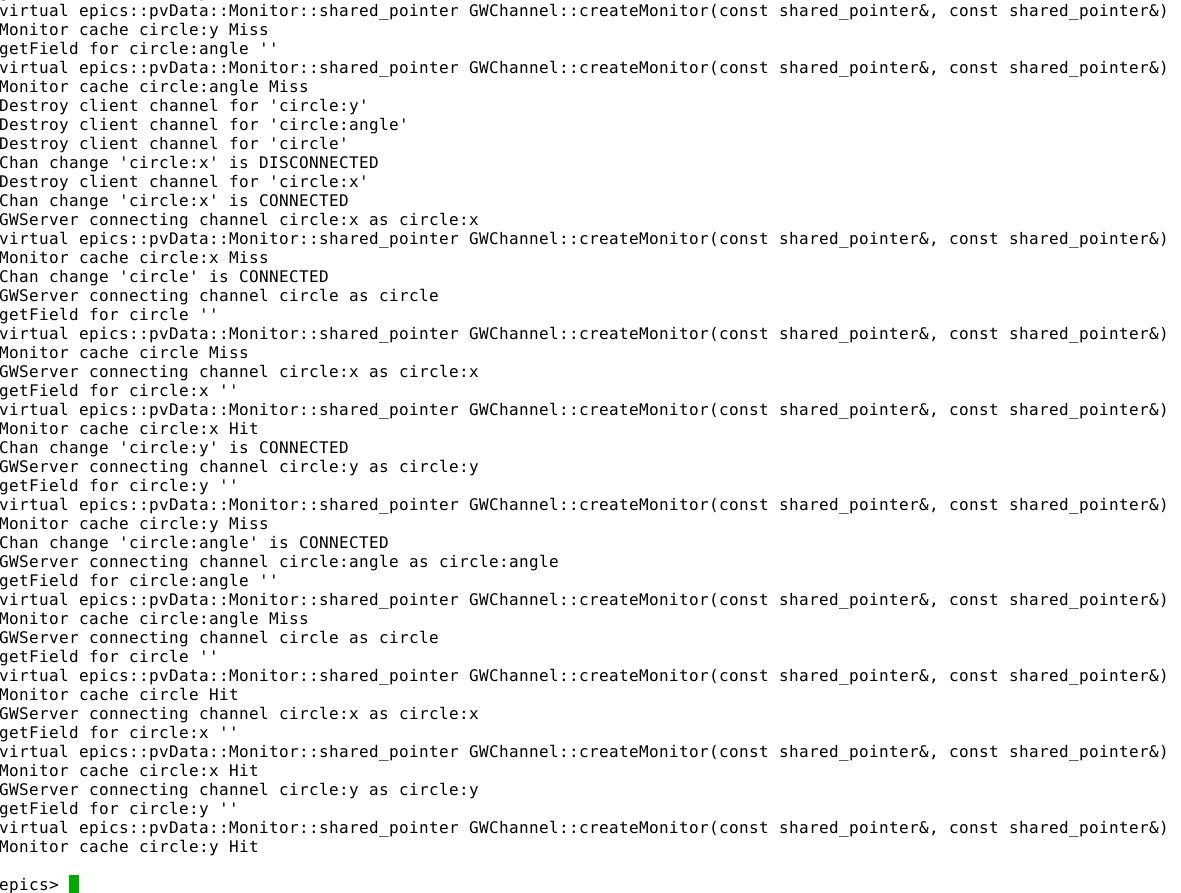
\includegraphics[width=0.8\textwidth, height=0.5\textheight]{./images/gw_msg.png}
	\caption{
		Gateway Message
	}		
	\label{fig:gw_msg}   
\end{figure}

\clearpage
\section{용어}
\subsubsection{IP}
Internet Protocol (v4 and/or v6)

\subsubsection{PV}
Process Variable. Addressable unit in PVA.

\subsubsection{PVA}
PVAccess network protocol

\subsubsection{GW}
Gateway

\subsubsection{CLI}
An arbitrary PVAccess client (end user or another gateway)

\subsubsection{GWS}
Gateway server side (CLI communicates with this)

\subsubsection{GWC}
Gateway client side (SRV communicates with this)

\subsubsection{SRV}
An arbitrary PVAccess EPICS IOC server (may be another gateway)



\clearpage
\bibliographystyle{unsrtnat}
\bibliography{./refs}

\newpage
\appendix
\newappendix
\label{app:code_list}

\section{EPICS V4 PVAccess 및 PVAccess Gateway Code List}
\begin{lstlisting}[style=termstylenumber, caption={Code List}, label={list:nfsroot-file}]
pva2pva/p2pApp/server.cpp
pva2pva/p2pApp/main.cpp
pva2pva/p2pApp/client.cpp
pva2pva/p2pApp/chancache.cpp
pva2pva/p2pApp/moncache.cpp
pva2pva/p2pApp/channel.cpp
pva2pva/pdbApp/pvif.cpp
pva2pva/pdbApp/pdb.cpp
pva2pva/pdbApp/qsrv.cpp
pva2pva/pdbApp/pvalink.cpp
pva2pva/pdbApp/softMain.cpp
pva2pva/pdbApp/pdbsingle.cpp
pva2pva/pdbApp/pdbgroup.cpp
pvAccess/pvtoolsSrc/pvutils.cpp
pvAccess/pvtoolsSrc/pvlist.cpp
pvAccess/pvtoolsSrc/pvput.cpp
pvAccess/pvtoolsSrc/eget.cpp
pvAccess/pvtoolsSrc/pvinfo.cpp
pvAccess/pvtoolsSrc/pvget.cpp
pvAccess/src/factory/ChannelAccessFactory.cpp
pvAccess/src/remoteClient/clientContextImpl.cpp
pvAccess/src/ca/caStatus.cpp
pvAccess/src/ca/caProvider.cpp
pvAccess/src/ca/caChannel.cpp
pvAccess/src/mb/pvAccessMB.cpp
pvAccess/src/client/pvAccess.cpp
pvAccess/src/rpcService/rpcService.cpp
pvAccess/src/rpcService/rpcServer.cpp
pvAccess/src/remote/security.cpp
pvAccess/src/remote/codec.cpp
pvAccess/src/remote/transportRegistry.cpp
pvAccess/src/remote/blockingUDPConnector.cpp
pvAccess/src/remote/serializationHelper.cpp
pvAccess/src/remote/simpleChannelSearchManagerImpl.cpp
pvAccess/src/remote/blockingTCPAcceptor.cpp
pvAccess/src/remote/blockingUDPTransport.cpp
pvAccess/src/remote/beaconHandler.cpp
pvAccess/src/remote/abstractResponseHandler.cpp
pvAccess/src/remote/blockingTCPConnector.cpp
pvAccess/src/pipelineService/pipelineService.cpp
pvAccess/src/pipelineService/pipelineServer.cpp
pvAccess/src/server/serverContext.cpp
pvAccess/src/server/beaconServerStatusProvider.cpp
pvAccess/src/server/beaconEmitter.cpp
pvAccess/src/server/serverChannelImpl.cpp
pvAccess/src/server/baseChannelRequester.cpp
pvAccess/src/server/responseHandlers.cpp
pvAccess/src/utils/wildcard.cpp
pvAccess/src/utils/inetAddressUtil.cpp
pvAccess/src/utils/referenceCountingLock.cpp
pvAccess/src/utils/introspectionRegistry.cpp
pvAccess/src/utils/configuration.cpp
pvAccess/src/utils/hexDump.cpp
pvAccess/src/utils/logger.cpp
pvAccess/src/ioc/PVAClientRegister.cpp
pvAccess/src/ioc/PVAServerRegister.cpp
pvAccess/src/pva/clientFactory.cpp
pvAccess/src/pva/pvaVersion.cpp
pvAccess/src/rpcClient/rpcClient.cpp
pvaPy/src/pvaccess/PvAlarm.cpp
pvaPy/src/pvaccess/pvaccess.PvLong.cpp
pvaPy/src/pvaccess/PvaExceptionTranslator.cpp
pvaPy/src/pvaccess/RpcChannelProviderFactory.cpp
pvaPy/src/pvaccess/Channel.440.cpp
pvaPy/src/pvaccess/pvaccess.Channel.cpp
pvaPy/src/pvaccess/PvFloat.cpp
pvaPy/src/pvaccess/pvaccess.NtType.cpp
pvaPy/src/pvaccess/PvUShort.cpp
pvaPy/src/pvaccess/NtTable.cpp
pvaPy/src/pvaccess/pvaccess.PvObject.cpp
pvaPy/src/pvaccess/pvaccess.PvTimeStamp.cpp
pvaPy/src/pvaccess/InvalidArgument.cpp
pvaPy/src/pvaccess/PvaClient.cpp
pvaPy/src/pvaccess/PvShort.cpp
pvaPy/src/pvaccess/pvaccess.PvUShort.cpp
pvaPy/src/pvaccess/PvaPyLogger.cpp
pvaPy/src/pvaccess/ChannelMonitorRequesterImpl.cpp
pvaPy/src/pvaccess/PvInt.cpp
pvaPy/src/pvaccess/NtType.cpp
pvaPy/src/pvaccess/Channel.450.cpp
pvaPy/src/pvaccess/PvUInt.cpp
pvaPy/src/pvaccess/pvaccess.PvBoolean.cpp
pvaPy/src/pvaccess/PvBoolean.cpp
pvaPy/src/pvaccess/PvDouble.cpp
pvaPy/src/pvaccess/ChannelGetRequesterImpl.cpp
pvaPy/src/pvaccess/PvProvider.cpp
pvaPy/src/pvaccess/PvUnion.cpp
pvaPy/src/pvaccess/pvaccess.NtTable.cpp
pvaPy/src/pvaccess/pvaccess.PvProvider.cpp
pvaPy/src/pvaccess/pvaccess.RpcClient.cpp
pvaPy/src/pvaccess/pvaccess.PvULong.cpp
pvaPy/src/pvaccess/InvalidDataType.cpp
pvaPy/src/pvaccess/RpcTimeout.cpp
pvaPy/src/pvaccess/PvScalar.cpp
pvaPy/src/pvaccess/PvaException.cpp
pvaPy/src/pvaccess/ChannelPutRequesterImpl.cpp
pvaPy/src/pvaccess/ObjectNotFound.cpp
pvaPy/src/pvaccess/RpcChannelImpl.cpp
pvaPy/src/pvaccess/pvaccess.PvUInt.cpp
pvaPy/src/pvaccess/PvByte.cpp
pvaPy/src/pvaccess/RpcChannelProviderImpl.cpp
pvaPy/src/pvaccess/RpcClient.cpp
pvaPy/src/pvaccess/ConversionUtility.cpp
pvaPy/src/pvaccess/PvTimeStamp.cpp
pvaPy/src/pvaccess/pvaccess.PvFloat.cpp
pvaPy/src/pvaccess/PyGilManager.cpp
pvaPy/src/pvaccess/pvaccess.PvString.cpp
pvaPy/src/pvaccess/pvaccess.PvShort.cpp
pvaPy/src/pvaccess/PvaConstants.cpp
pvaPy/src/pvaccess/RpcServiceImpl.cpp
pvaPy/src/pvaccess/pvaccess.PvByte.cpp
pvaPy/src/pvaccess/pvaccess.cpp
pvaPy/src/pvaccess/PyUtility.cpp
pvaPy/src/pvaccess/PvLong.cpp
pvaPy/src/pvaccess/ChannelNotFound.cpp
pvaPy/src/pvaccess/pvaccess.PvType.cpp
pvaPy/src/pvaccess/RpcServerContextImpl.cpp
pvaPy/src/pvaccess/pvaccess.PvScalar.cpp
pvaPy/src/pvaccess/ChannelRpcServiceImpl.cpp
pvaPy/src/pvaccess/Channel.cpp
pvaPy/src/pvaccess/pvaccess.PvInt.cpp
pvaPy/src/pvaccess/pvaccess.RpcServer.cpp
pvaPy/src/pvaccess/FieldNotFound.cpp
pvaPy/src/pvaccess/pvaccess.PvAlarm.cpp
pvaPy/src/pvaccess/StringUtility.cpp
pvaPy/src/pvaccess/pvaccess.PvScalarArray.cpp
pvaPy/src/pvaccess/PyPvDataUtility.cpp
pvaPy/src/pvaccess/InvalidState.cpp
pvaPy/src/pvaccess/ChannelTimeout.cpp
pvaPy/src/pvaccess/pvaccess.PvUnion.cpp
pvaPy/src/pvaccess/CaClient.cpp
pvaPy/src/pvaccess/PvUByte.cpp
pvaPy/src/pvaccess/PvULong.cpp
pvaPy/src/pvaccess/RpcServer.cpp
pvaPy/src/pvaccess/RequesterImpl.cpp
pvaPy/src/pvaccess/PvString.cpp
pvaPy/src/pvaccess/PvScalarArray.cpp
pvaPy/src/pvaccess/GetFieldRequesterImpl.cpp
pvaPy/src/pvaccess/pvaccess.PvDouble.cpp
pvaPy/src/pvaccess/ChannelRequesterImpl.cpp
pvaPy/src/pvaccess/InvalidRequest.cpp
pvaPy/src/pvaccess/PvObject.cpp
pvaPy/src/pvaccess/pvaccess.PvUByte.cpp
pvaPy/src/pvaccess/PvUtility.cpp
pvaSrv/exampleTop/simpleDbPv/src/simpleDbPvMain.cpp
pvaSrv/exampleTop/simpleDbPv/src/O.linux-x86_64/simpleDbPv_registerRecordDeviceDriver.cpp
pvaSrv/src/dbPv/3.15/caSecurity.cpp
pvaSrv/src/dbPv/3.15/dbPvMonitor.cpp
pvaSrv/src/dbPv/3.15/caMonitor.cpp
pvaSrv/src/dbPv/3.15/caContext.cpp
pvaSrv/src/dbPv/3.15/dbPvGet.cpp
pvaSrv/src/dbPv/3.15/dbPvProcess.cpp
pvaSrv/src/dbPv/3.15/dbPvArray.cpp
pvaSrv/src/dbPv/3.15/dbUtil.cpp
pvaSrv/src/dbPv/3.15/dbPv.cpp
pvaSrv/src/dbPv/3.15/dbPvPut.cpp
pvaSrv/src/dbPv/3.15/dbPvProvider.cpp
pvaSrv/src/dbPv/3.15/dbPvRegister.cpp
pvaSrv/src/dbPv/3.14/caSecurity.cpp
pvaSrv/src/dbPv/3.14/dbPvMonitor.cpp
pvaSrv/src/dbPv/3.14/caMonitor.cpp
pvaSrv/src/dbPv/3.14/caContext.cpp
pvaSrv/src/dbPv/3.14/dbPvGet.cpp
pvaSrv/src/dbPv/3.14/dbPvProcess.cpp
pvaSrv/src/dbPv/3.14/dbPvArray.cpp
pvaSrv/src/dbPv/3.14/dbUtil.cpp
pvaSrv/src/dbPv/3.14/dbPv.cpp
pvaSrv/src/dbPv/3.14/dbPvPut.cpp
pvaSrv/src/dbPv/3.14/dbPvProvider.cpp
pvaSrv/src/dbPv/3.14/dbPvRegister.cpp
pvaSrv/src/dbGroup/dbGroupProvider.cpp
pvaSrv/src/dbGroup/dbGroup.cpp
pvaSrv/src/dbGroup/pvValue.cpp
pvaSrv/src/dbGroup/dbGroupRegister.cpp
pvaSrv/src/dbGroup/dbGroupGet.cpp
pvaSrv/src/softMain.cpp
pvaSrv/src/O.linux-x86_64/softIocPVA_registerRecordDeviceDriver.cpp
pvData/src/factory/PVUnionArray.cpp
pvData/src/factory/PVDataCreateFactory.cpp
pvData/src/factory/Compare.cpp
pvData/src/factory/TypeFunc.cpp
pvData/src/factory/PVStructureArray.cpp
pvData/src/factory/pvSubArrayCopy.cpp
pvData/src/factory/PVUnion.cpp
pvData/src/factory/FieldCreateFactory.cpp
pvData/src/factory/PVArray.cpp
pvData/src/factory/PVScalarArray.cpp
pvData/src/factory/StandardPVField.cpp
pvData/src/factory/PVField.cpp
pvData/src/factory/PVStructure.cpp
pvData/src/factory/PVScalar.cpp
pvData/src/factory/printer.cpp
pvData/src/factory/Convert.cpp
pvData/src/factory/StandardField.cpp
pvData/src/pvMisc/bitSetUtil.cpp
pvData/src/property/pvControl.cpp
pvData/src/property/pvTimeStamp.cpp
pvData/src/property/pvAlarm.cpp
pvData/src/property/timeStamp.cpp
pvData/src/property/alarm.cpp
pvData/src/property/pvEnumerated.cpp
pvData/src/property/pvDisplay.cpp
pvData/src/misc/event.cpp
pvData/src/misc/byteBuffer.cpp
pvData/src/misc/typeCast.cpp
pvData/src/misc/parseToPOD.cpp
pvData/src/misc/serializeHelper.cpp
pvData/src/misc/bitSet.cpp
pvData/src/misc/status.cpp
pvData/src/misc/requester.cpp
pvData/src/misc/epicsException.cpp
pvData/src/misc/localStaticLock.cpp
pvData/src/misc/messageQueue.cpp
pvData/src/misc/timer.cpp
pvData/src/misc/executor.cpp
pvData/src/misc/timeFunction.cpp
pvData/src/copy/pvCopy.cpp
pvData/src/copy/createRequest.cpp
pvData/src/monitor/monitor.cpp
pvData/src/monitor/monitorPlugin.cpp
pvaClient/src/pvaClientMultiChannel.cpp
pvaClient/src/pvaClientProcess.cpp
pvaClient/src/pvaClientChannel.cpp
pvaClient/src/pvaClientMonitorData.cpp
pvaClient/src/pvaClientMultiPutDouble.cpp
pvaClient/src/pvaClientMultiMonitorDouble.cpp
pvaClient/src/pvaClientNTMultiData.cpp
pvaClient/src/pvaClientPutData.cpp
pvaClient/src/pvaClientGet.cpp
pvaClient/src/pvaClientNTMultiMonitor.cpp
pvaClient/src/pvaClientMonitor.cpp
pvaClient/src/pvaClientNTMultiPut.cpp
pvaClient/src/pvaClientGetData.cpp
pvaClient/src/pvaClientPut.cpp
pvaClient/src/pvaClient.cpp
pvaClient/src/pvaClientPutGet.cpp
pvaClient/src/pvaClientMultiGetDouble.cpp
pvaClient/src/pvaClientNTMultiGet.cpp
normativeTypes/src/nt/ntmultiChannel.cpp
normativeTypes/src/nt/ntid.cpp
normativeTypes/src/nt/nthistogram.cpp
normativeTypes/src/nt/ntndarrayAttribute.cpp
normativeTypes/src/nt/ntmatrix.cpp
normativeTypes/src/nt/ntscalar.cpp
normativeTypes/src/nt/nturi.cpp
normativeTypes/src/nt/ntnameValue.cpp
normativeTypes/src/nt/ntutils.cpp
normativeTypes/src/nt/ntunion.cpp
normativeTypes/src/nt/ntaggregate.cpp
normativeTypes/src/nt/ntcontinuum.cpp
normativeTypes/src/nt/nttable.cpp
normativeTypes/src/nt/ntattribute.cpp
normativeTypes/src/nt/ntscalarArray.cpp
normativeTypes/src/nt/ntndarray.cpp
normativeTypes/src/nt/ntenum.cpp
normativeTypes/src/nt/ntscalarMultiChannel.cpp
normativeTypes/src/nt/ntfield.cpp
pva2pva/common/pvatypemap.h
pva2pva/common/pvahelper.h
pva2pva/common/errlogstream.h
pva2pva/p2pApp/iocshelper.h
pva2pva/p2pApp/weakset.h
pva2pva/p2pApp/pva2pva.h
pva2pva/p2pApp/helper.h
pva2pva/p2pApp/chancache.h
pva2pva/p2pApp/weakmap.h
pva2pva/p2pApp/channel.h
pva2pva/p2pApp/server.h
pva2pva/pdbApp/pdb.h
pva2pva/pdbApp/pdbgroup.h
pva2pva/pdbApp/pdbsingle.h
pva2pva/pdbApp/pvif.h
pvAccess/include/pv/syncChannelFind.h
pvAccess/include/pv/rpcClient.h
pvAccess/include/pv/pipelineServer.h
pvAccess/include/pv/inetAddressUtil.h
pvAccess/include/pv/beaconServerStatusProvider.h
pvAccess/include/pv/namedLockPattern.h
pvAccess/include/pv/serializationHelper.h
pvAccess/include/pv/caChannel.h
pvAccess/include/pv/responseHandlers.h
pvAccess/include/pv/caStatus.h
pvAccess/include/pv/pvAccess.h
pvAccess/include/pv/hexDump.h
pvAccess/include/pv/pipelineService.h
pvAccess/include/pv/beaconHandler.h
pvAccess/include/pv/configuration.h
pvAccess/include/pv/codec.h
pvAccess/include/pv/baseChannelRequester.h
pvAccess/include/pv/blockingUDP.h
pvAccess/include/pv/introspectionRegistry.h
pvAccess/include/pv/logger.h
pvAccess/include/pv/fairQueue.h
pvAccess/include/pv/referenceCountingLock.h
pvAccess/include/pv/security.h
pvAccess/include/pv/simpleChannelSearchManagerImpl.h
pvAccess/include/pv/pvaConstants.h
pvAccess/include/pv/caProvider.h
pvAccess/include/pv/pvaVersion.h
pvAccess/include/pv/serverChannelImpl.h
pvAccess/include/pv/blockingTCP.h
pvAccess/include/pv/remote.h
pvAccess/include/pv/pvAccessMB.h
pvAccess/include/pv/beaconEmitter.h
pvAccess/include/pv/rpcService.h
pvAccess/include/pv/transportRegistry.h
pvAccess/include/pv/wildcard.h
pvAccess/include/pv/channelSearchManager.h
pvAccess/include/pv/rpcServer.h
pvAccess/include/pv/pvaVersionNum.h
pvAccess/include/pv/clientFactory.h
pvAccess/include/pv/serverContext.h
pvAccess/include/pv/clientContextImpl.h
pvAccess/include/pv/likely.h
pvAccess/pvtoolsSrc/pvutils.h
pvAccess/src/remoteClient/pv/clientContextImpl.h
pvAccess/src/ca/pv/caChannel.h
pvAccess/src/ca/pv/caStatus.h
pvAccess/src/ca/pv/caProvider.h
pvAccess/src/mb/pv/pvAccessMB.h
pvAccess/src/client/pv/pvAccess.h
pvAccess/src/rpcService/pv/rpcService.h
pvAccess/src/rpcService/pv/rpcServer.h
pvAccess/src/remote/pv/serializationHelper.h
pvAccess/src/remote/pv/beaconHandler.h
pvAccess/src/remote/pv/codec.h
pvAccess/src/remote/pv/blockingUDP.h
pvAccess/src/remote/pv/security.h
pvAccess/src/remote/pv/simpleChannelSearchManagerImpl.h
pvAccess/src/remote/pv/blockingTCP.h
pvAccess/src/remote/pv/remote.h
pvAccess/src/remote/pv/transportRegistry.h
pvAccess/src/remote/pv/channelSearchManager.h
pvAccess/src/pipelineService/pv/pipelineServer.h
pvAccess/src/pipelineService/pv/pipelineService.h
pvAccess/src/server/pv/beaconServerStatusProvider.h
pvAccess/src/server/pv/responseHandlers.h
pvAccess/src/server/pv/baseChannelRequester.h
pvAccess/src/server/pv/serverChannelImpl.h
pvAccess/src/server/pv/beaconEmitter.h
pvAccess/src/server/pv/serverContext.h
pvAccess/src/utils/pv/inetAddressUtil.h
pvAccess/src/utils/pv/namedLockPattern.h
pvAccess/src/utils/pv/hexDump.h
pvAccess/src/utils/pv/configuration.h
pvAccess/src/utils/pv/introspectionRegistry.h
pvAccess/src/utils/pv/logger.h
pvAccess/src/utils/pv/fairQueue.h
pvAccess/src/utils/pv/referenceCountingLock.h
pvAccess/src/utils/pv/wildcard.h
pvAccess/src/utils/pv/likely.h
pvAccess/src/ioc/pv/syncChannelFind.h
pvAccess/src/O.Common/pv/pvaVersionNum.h
pvAccess/src/pva/pv/pvaConstants.h
pvAccess/src/pva/pv/pvaVersion.h
pvAccess/src/pva/pv/clientFactory.h
pvAccess/src/rpcClient/pv/rpcClient.h
pvaPy/src/pvaccess/PvaException.h
pvaPy/src/pvaccess/PvUInt.h
pvaPy/src/pvaccess/PvaConstants.h
pvaPy/src/pvaccess/PyUtility.h
pvaPy/src/pvaccess/RpcChannelImpl.h
pvaPy/src/pvaccess/RpcServer.h
pvaPy/src/pvaccess/ChannelRequesterImpl.h
pvaPy/src/pvaccess/PvUShort.h
pvaPy/src/pvaccess/RpcServerContextImpl.h
pvaPy/src/pvaccess/ConversionUtility.h
pvaPy/src/pvaccess/PvaPyLogger.h
pvaPy/src/pvaccess/PvShort.h
pvaPy/src/pvaccess/PvScalar.h
pvaPy/src/pvaccess/PvObject.h
pvaPy/src/pvaccess/NtTable.h
pvaPy/src/pvaccess/PvBoolean.h
pvaPy/src/pvaccess/InvalidDataType.h
pvaPy/src/pvaccess/ChannelRpcServiceImpl.h
pvaPy/src/pvaccess/PyGilManager.h
pvaPy/src/pvaccess/RpcTimeout.h
pvaPy/src/pvaccess/InvalidState.h
pvaPy/src/pvaccess/RequesterImpl.h
pvaPy/src/pvaccess/PyPvDataUtility.h
pvaPy/src/pvaccess/ChannelMonitorRequesterImpl.h
pvaPy/src/pvaccess/PvLong.h
pvaPy/src/pvaccess/RpcChannelProviderFactory.h
pvaPy/src/pvaccess/PvType.h
pvaPy/src/pvaccess/ChannelGetRequesterImpl.h
pvaPy/src/pvaccess/InvalidArgument.h
pvaPy/src/pvaccess/PvProvider.h
pvaPy/src/pvaccess/RpcClient.h
pvaPy/src/pvaccess/NtType.h
pvaPy/src/pvaccess/PvULong.h
pvaPy/src/pvaccess/AtomicBool.h
pvaPy/src/pvaccess/PvUtility.h
pvaPy/src/pvaccess/PvAlarm.h
pvaPy/src/pvaccess/PvUnion.h
pvaPy/src/pvaccess/PvaClient.h
pvaPy/src/pvaccess/Channel.450.h
pvaPy/src/pvaccess/StringUtility.h
pvaPy/src/pvaccess/PvScalarArray.h
pvaPy/src/pvaccess/Channel.h
pvaPy/src/pvaccess/PvaExceptionTranslator.h
pvaPy/src/pvaccess/PyGilRelease.h
pvaPy/src/pvaccess/PvTimeStamp.h
pvaPy/src/pvaccess/PvString.h
pvaPy/src/pvaccess/Channel.440.h
pvaPy/src/pvaccess/PvaClientUtility.h
pvaPy/src/pvaccess/ChannelNotFound.h
pvaPy/src/pvaccess/RpcServiceImpl.h
pvaPy/src/pvaccess/PvUByte.h
pvaPy/src/pvaccess/FieldNotFound.h
pvaPy/src/pvaccess/ObjectNotFound.h
pvaPy/src/pvaccess/ChannelPutRequesterImpl.h
pvaPy/src/pvaccess/PvFloat.h
pvaPy/src/pvaccess/PvByte.h
pvaPy/src/pvaccess/CaClient.h
pvaPy/src/pvaccess/InvalidRequest.h
pvaPy/src/pvaccess/SynchronizedQueue.h
pvaPy/src/pvaccess/RpcChannelProviderImpl.h
pvaPy/src/pvaccess/ChannelTimeout.h
pvaPy/src/pvaccess/PvDouble.h
pvaPy/src/pvaccess/GetFieldRequesterImpl.h
pvaPy/src/pvaccess/PvInt.h
pvaSrv/include/caMonitor.h
pvaSrv/include/dbPv.h
pvaSrv/include/caSecurity.h
pvaSrv/include/dbPvDebug.h
pvaSrv/src/dbPv/3.15/caContext.h
pvaSrv/src/dbPv/3.15/caMonitor.h
pvaSrv/src/dbPv/3.15/dbPv.h
pvaSrv/src/dbPv/3.15/caSecurity.h
pvaSrv/src/dbPv/3.15/dbUtil.h
pvaSrv/src/dbPv/3.15/dbPvDebug.h
pvaSrv/src/dbPv/3.14/caContext.h
pvaSrv/src/dbPv/3.14/caMonitor.h
pvaSrv/src/dbPv/3.14/dbPv.h
pvaSrv/src/dbPv/3.14/caSecurity.h
pvaSrv/src/dbPv/3.14/dbUtil.h
pvaSrv/src/dbPv/3.14/dbPvDebug.h
pvaSrv/src/dbGroup/dbGroup.h
pvaSrv/src/dbGroup/pvValue.h
pvData/include/pv/thread.h
pvData/include/pv/createRequest.h
pvData/include/pv/factory.h
pvData/include/pv/pvSubArrayCopy.h
pvData/include/pv/timeStamp.h
pvData/include/pv/localStaticLock.h
pvData/include/pv/sharedVector.h
pvData/include/pv/epicsException.h
pvData/include/pv/pvControl.h
pvData/include/pv/pvTimeStamp.h
pvData/include/pv/display.h
pvData/include/pv/requester.h
pvData/include/pv/monitor.h
pvData/include/pv/sharedPtr.h
pvData/include/pv/pvEnumerated.h
pvData/include/pv/destroyable.h
pvData/include/pv/serialize.h
pvData/include/pv/pvData.h
pvData/include/pv/convert.h
pvData/include/pv/monitorPlugin.h
pvData/include/pv/event.h
pvData/include/pv/messageQueue.h
pvData/include/pv/byteBuffer.h
pvData/include/pv/status.h
pvData/include/pv/pvAlarm.h
pvData/include/pv/standardField.h
pvData/include/pv/queue.h
pvData/include/pv/bitSet.h
pvData/include/pv/serializeHelper.h
pvData/include/pv/executor.h
pvData/include/pv/timeFunction.h
pvData/include/pv/noDefaultMethods.h
pvData/include/pv/lock.h
pvData/include/pv/typeCast.h
pvData/include/pv/pvType.h
pvData/include/pv/control.h
pvData/include/pv/pvCopy.h
pvData/include/pv/alarm.h
pvData/include/pv/bitSetUtil.h
pvData/include/pv/standardPVField.h
pvData/include/pv/pvIntrospect.h
pvData/include/pv/pvDisplay.h
pvData/include/pv/current_function.h
pvData/include/pv/templateMeta.h
pvData/include/pv/timer.h
pvData/src/factory/pv/factory.h
pvData/src/pvMisc/pv/bitSetUtil.h
pvData/src/property/pv/timeStamp.h
pvData/src/property/pv/pvControl.h
pvData/src/property/pv/pvTimeStamp.h
pvData/src/property/pv/display.h
pvData/src/property/pv/pvEnumerated.h
pvData/src/property/pv/pvAlarm.h
pvData/src/property/pv/control.h
pvData/src/property/pv/alarm.h
pvData/src/property/pv/pvDisplay.h
pvData/src/pv/pvSubArrayCopy.h
pvData/src/pv/pvData.h
pvData/src/pv/convert.h
pvData/src/pv/standardField.h
pvData/src/pv/pvType.h
pvData/src/pv/standardPVField.h
pvData/src/pv/pvIntrospect.h
pvData/src/misc/pv/thread.h
pvData/src/misc/pv/localStaticLock.h
pvData/src/misc/pv/sharedVector.h
pvData/src/misc/pv/epicsException.h
pvData/src/misc/pv/requester.h
pvData/src/misc/pv/sharedPtr.h
pvData/src/misc/pv/destroyable.h
pvData/src/misc/pv/serialize.h
pvData/src/misc/pv/event.h
pvData/src/misc/pv/messageQueue.h
pvData/src/misc/pv/byteBuffer.h
pvData/src/misc/pv/status.h
pvData/src/misc/pv/queue.h
pvData/src/misc/pv/bitSet.h
pvData/src/misc/pv/serializeHelper.h
pvData/src/misc/pv/executor.h
pvData/src/misc/pv/timeFunction.h
pvData/src/misc/pv/noDefaultMethods.h
pvData/src/misc/pv/lock.h
pvData/src/misc/pv/typeCast.h
pvData/src/misc/pv/current_function.h
pvData/src/misc/pv/templateMeta.h
pvData/src/misc/pv/timer.h
pvData/src/copy/pv/createRequest.h
pvData/src/copy/pv/pvCopy.h
pvData/src/monitor/pv/monitor.h
pvData/src/monitor/pv/monitorPlugin.h
pvaClient/include/pv/pvaClient.h
pvaClient/include/pv/pvaClientMultiChannel.h
pvaClient/src/pv/pvaClient.h
pvaClient/src/pv/pvaClientMultiChannel.h
normativeTypes/include/pv/ntunion.h
normativeTypes/include/pv/ntndarrayAttribute.h
normativeTypes/include/pv/ntscalarArray.h
normativeTypes/include/pv/nt.h
normativeTypes/include/pv/ntenum.h
normativeTypes/include/pv/ntutils.h
normativeTypes/include/pv/nttable.h
normativeTypes/include/pv/ntndarray.h
normativeTypes/include/pv/ntscalar.h
normativeTypes/include/pv/ntmatrix.h
normativeTypes/include/pv/nthistogram.h
normativeTypes/include/pv/nturi.h
normativeTypes/include/pv/ntid.h
normativeTypes/include/pv/ntscalarMultiChannel.h
normativeTypes/include/pv/ntmultiChannel.h
normativeTypes/include/pv/ntaggregate.h
normativeTypes/include/pv/ntfield.h
normativeTypes/include/pv/ntnameValue.h
normativeTypes/include/pv/ntcontinuum.h
normativeTypes/include/pv/ntattribute.h
normativeTypes/src/nt/ntunion.h
normativeTypes/src/nt/ntndarrayAttribute.h
normativeTypes/src/nt/ntscalarArray.h
normativeTypes/src/nt/nt.h
normativeTypes/src/nt/ntenum.h
normativeTypes/src/nt/ntutils.h
normativeTypes/src/nt/nttable.h
normativeTypes/src/nt/ntndarray.h
normativeTypes/src/nt/ntscalar.h
normativeTypes/src/nt/ntmatrix.h
normativeTypes/src/nt/nthistogram.h
normativeTypes/src/nt/nturi.h
normativeTypes/src/nt/ntid.h
normativeTypes/src/nt/ntscalarMultiChannel.h
normativeTypes/src/nt/ntmultiChannel.h
normativeTypes/src/nt/ntaggregate.h
normativeTypes/src/nt/ntfield.h
normativeTypes/src/nt/ntnameValue.h
normativeTypes/src/nt/ntcontinuum.h
normativeTypes/src/nt/ntattribute.h
\end{lstlisting}
\end{document}

